\documentclass[11pt]{article}
\usepackage[left=25mm,right=25mm,top=30mm,bottom=30mm]{geometry}
\usepackage{amsmath} % math
\usepackage{amssymb} % math
\usepackage{graphicx} % to use \includegraphics{}
\usepackage{amsthm}
\usepackage{diagbox} % to make tables
\usepackage{kotex} % to use korean(hangul)
\usepackage{caption}
\usepackage[hidelinks]{hyperref}
\usepackage[group-separator={,}]{siunitx} %si unit
% \usepackage[hangul]{kotex} 이걸로하면 Abstract, Contents 등이 전부 요약, 내용 등으로 바뀜.

\pagenumbering{roman} % \pagenumbering{다른거}나올때까지 roman으로 
%pagenumbering.

\renewcommand\thesection{\Roman{section}} % \section : In roman(I,II,III,...)
\renewcommand\thesubsection{\arabic{subsection}} % \subsection : In 
%arabic(1,2,3,...)

\usepackage{chngcntr}
\renewcommand\thesubsubsection{%
	\thesubsection.\arabic{subsubsection}%
}
\usepackage{titlesec}
\titlelabel{\thetitle.\quad}
%subsubsection에 점이 두 개씩 찍히는 것을 막고,
%점이 문단 번호에만 찍히도록 수정.

\usepackage{tocloft}%
\setlength{\cftsecnumwidth}{3em}% 
\setlength{\cftsubsecnumwidth}{1em}%
\setlength{\cftsubsubsecnumwidth}{2em}%
%toc의 여백 조정으로 VIII와 같은 번호가 제목과 겹치는 것을 방지


\newtheorem{definition}{정의}
\newtheorem{collorary}{보조정리}
\newtheorem{praise}{찬양}

\begin{document}

\begin{center}
	\Large An Introduction to \LaTeX
	\small especially for GSHS students
\end{center}

\begin{abstract}
	
	\begin{large}
	An-Introduction-to-LaTeX
	\end{large}

	논문작성을 위한 LaTeX 입문서를 LaTeX로 제작한 것입니다.
	
	LaTeX Editor로는 TeXstudio를 추천합니다. 개인적으로 쓰고 있는 것이기도 해서...
	
	http://www.texstudio.org/
	
	TeXworks쓰다가 TeXstudio쓰면 정말 내가 왜 이걸 모르고 있었지 싶음...
	
	TeX에서 한글을 사용하기 위해서는 koTeXlive를 별도로 설치해야 합니다.
	
	www.ktug.org/xe/index.php?mid=install
	
	용량이 1GB정도 되니 주의 바람
	
	\bigskip
	
	웹사이트가 개설되었습니다! 새로운 버전이 생길 때마다 자동으로 업로드됩니다. 
	
	\href{http://gshslatexintro.github.io/gshslatexintro/}{Download Page}
	
	\begin{praise}
		HLETRD는 31기 선배들 중 \LaTeX 의 최고수이시다.
		저희 32기에게 처음 \LaTeX 를 가르쳐 주시고 class 파일도 
		만들어주신 정민석 선생님께 감사드립니다.
	\end{praise}
	
	\bigskip
	
	\textbf{우리의 기초 R\&E는 수학 R\&E가 아닌 LaTeX R\&E이었습니다.}
	
	\bigskip
	
	\begin{flushright}
		-익명
	\end{flushright}
\end{abstract}
%강제개행으로 두 줄을 띄면 overfull 경고 발생. medskip이나 bigskip 이용.

\clearpage
\tableofcontents

\clearpage
\listoftables

\clearpage
\listoffigures

\clearpage
\newcommand{\ding}{\textit{Sample figure}}
\newcommand{\longline}{=================================}

%roman numbering for sections
%\renewcommand\thesection{\Roman{section}.}
%\renewcommand\thesubsection{\arabic{subsection}.
\pagenumbering{arabic}

\section{What is \LaTeX ? How to install?}\label{intro}
우리는 보통 논문이나 R\&E보고서를 작성할 때 아래아한글이나 MS워드를 사용하곤 한다. 하지만 논문의 가독성 향상, 그림/표 넘버링과 간편한 리스트 작성을 위해 보통 대학원 이상에서는 \LaTeX 를 사용하곤 한다. 

더욱 자세한 내용을 알고 싶다면 namu.wiki/w/LaTeX 을 읽어보길 추천한다.

TeX을 사용하기 위해서는 Editor가 필요하다.
Windows의 경우 (무료) TeXworks, TeXstudio, TeXnicCenter 등이 있다. 개인적으로는 처음 배울때 TeXworks를 사용했었으나 뒤늦게 TeXstudio의 편리함을 깨우쳤다. TeXworks는 비추.

또한, 논문에 한글을 조금이라도 넣기 위해서는 kotexlive가 필요하다. 
www.ktug.org/xe/install 에서 다운받을 수 있다. 다만 용량이 1~GB 정도이니 데이터 
주의.

참고로 kotexlive를 최초로 만드신 분이 경기과학고 출신이시다.ㅎㅎ 

\section{Basic functions of \LaTeX}
\subsection{header}
\LaTeX 문서도 C언어 프로그래밍과 같이 헤더를 필요로 한다. 사용할 라이브러리를 import해줘야 되고, 필요한 command들을 지정할 때 주로 문서의 맨 앞부분에 쓰고는 한다. 어디까지가 헤더라고 명확히 말할 수는 없지만, 이 문서의 헤더를 쓰면 다음과 같다.

\subsection{High 가독성}
\LaTeX 를 이용하여 문서를 작성하게 될 경우 작성 중 그리고 읽을 때 모두 가독성이 높다.
작성 중에는 엔터를 두번 쳐야 실제로 줄이 넘어간다. 강제로 줄을 바꾸고 싶을 경우에는 \textbackslash \textbackslash 를 사용하면 된다.

\subsection{\textbackslash ref}

이것이 \ref{intro} 절에서 말하였던 기능이다.

\section{making tables}
\subsection{easy table : using \textbackslash hline}

\verb+\+begin\{table\}[h]

\verb+\+begin\{center\}

\verb+\+begin\{tabular\}\{\textbar c\textbar c\textbar c\textbar\}

\verb+\+hline

\verb+\+end\{tabular\}

\verb+\+end\{center\}

\verb+\+end\{table\}


\begin{table}[h]
	\begin{center}
		\begin{tabular}{|c|c|c|}
			\hline
		\end{tabular}
	\end{center}
\end{table}

이것은 표 삽입의 간단한 예제입니다.

표는 다음과 같이 삽입할 수 있다.

\verb+\+begin\{table\}[h]

\verb+\+begin\{center\}

\verb+\+begin\{tabular\}\{\textbar c\textbar c\textbar c\textbar\}

\verb+\+hline

학번\&이름\&특징\verb+\+\verb+\+

\verb+\+hline

\verb+\+hline

14012\&홍길동\&호부호형X\verb+\+\verb+\+

\verb+\+hline

12320\&전우치\&도술에 재능이 있음\verb+\+\verb+\+

\verb+\+hline

\verb+\+end\{tabular\}

\verb+\+end\{center\}

\verb+\+end\{table\}


\begin{table}[!h]
	\begin{center}
		\begin{tabular}{|c|c|c|}
			\hline
			학번&이름&특징\\
			\hline
			\hline
			14012&홍길동&호부호형X\\
			\hline
			12320&전우치&도술에 재능이 있음\\
			\hline
		\end{tabular}
	\end{center}
\end{table}

\longline

\verb+\+begin\{table\}[h]

\verb+\+begin\{center\}

\verb+\+begin\{tabular\}\{\textbar c\textbar c\textbar c\textbar\}

\verb+\+hline

학번\&이름\&특징\verb+\+\verb+\+

\verb+\+hline

14012\&홍길동\&ㅁㄴㅇㄹ\verb+\+\verb+\+

12320\&전우치\&도술\verb+\+\verb+\+

\verb+\+hline

\verb+\+end\{tabular\}

\verb+\+end\{center\}

\verb+\+end\{table\}

\begin{table}[!h]
	\begin{center}
		\begin{tabular}{c|c|c}
			\hline
			학번&이름&특징\\
			\hline
			14012&홍길동&ㅁㄴㅇㄹ\\
			12320&전우치&도술\\
			\hline
		\end{tabular}
	\end{center}
\end{table}

\subsection{using \textbackslash multirow}

\verb+\+begin\{table\}[h]

\verb+\+begin\{center\}

\verb+\+begin\{tabular\}\{\textbar c\textbar c\textbar c\textbar\}

\verb+\+hline

\verb+\+diagbox\{학년\}\{반\}\&1\&2\verb+\+\verb+\+

\verb+\+hline

\verb+\+hline

14012\&홍길동\&ㅁㄴㅇㄹ\verb+\+\verb+\+

12320\&전우치\&도술\verb+\+\verb+\+

\verb+\+hline

\verb+\+end\{tabular\}

\verb+\+end\{center\}

\verb+\+end\{table\}

\begin{table}[!h]
	\begin{center}
		\begin{tabular}{c|c|c}
			\hline
			\diagbox{학년}{반}&1&2\\
			\hline
			\hline
			14012&홍길동&ㅁㄴㅇㄹ\\
			12320&전우치&도술\\
			\hline
		\end{tabular}
	\end{center}
\end{table}

\longline

\verb+\+begin\{table\}[h]

\verb+\+begin\{center\}

\verb+\+begin\{tabular\}\{c\textbar c\textbar c\}

\verb+\+hline

\verb+\+multicolumn\{3\}\{c\}\{반장이름\}\verb+\+\verb+\+

\verb+\+diagbox\{학년\}\{반\}\&1\&2\verb+\+\verb+\+

\verb+\+hline

\verb+\+hline

14012\&홍길동\&ㅁㄴㅇㄹ\verb+\+\verb+\+

12320\&전우치\&도술\verb+\+\verb+\+

\verb+\+hline

\verb+\+end\{tabular\}

\verb+\+end\{center\}

\verb+\+end\{table\}

\begin{table}[!h]
	\begin{center}
	\begin{tabular}{c|c|c}
		\hline
		\multicolumn{3}{c}{반장이름}\\
		\diagbox{학년}{반}&1&2\\
		\hline
		\hline
		14012&홍길동&ㅁㄴㅇㄹ\\
		12320&전우치&도술\\
		\hline
		
	\end{tabular}
	\end{center}
\end{table}

\longline

\verb+\+begin\{table\}[h]

\verb+\+begin\{center\}

\verb+\+begin\{tabular\}\{\textbar c\textbar c\textbar c\textbar\}

\verb+\+hline

\&\verb+\+multicolumn\{2\}\{c\textbar\}\{반장이름\}\verb+\+\verb+\+

\verb+\+hline

\verb+\+diagbox\{학년\}\{반\}\&1\&2\verb+\+\verb+\+

\verb+\+hline

\verb+\+hline

14012\&홍길동\&ㅁㄴㅇㄹ\verb+\+\verb+\+

\verb+\+hline

12320\&전우치\&도술\verb+\+\verb+\+

\verb+\+hline

\verb+\+end\{tabular\}

\verb+\+caption\{1,2학년 반장\}\verb+\+label\{tab1\}

\verb+\+end\{center\}

\verb+\+end\{table\}

\begin{table}[!h]
	\begin{center}
	\begin{tabular}{|c|c|c|}
		\hline
		&\multicolumn{2}{c|}{반장이름}\\
		\hline
		\diagbox{학년}{반}&1&2\\
		\hline
		\hline
		14012&홍길동&ㅁㄴㅇㄹ\\
		\hline
		12320&전우치&도술\\
		\hline
	\end{tabular}
	\caption{sample table}\label{tab1}
	\end{center}
\end{table}

\section{Including images}
\subsection{first}

\verb+\+begin\{figure\}

\verb+\+begin\{center\}

\verb+\+includegraphics[scale=0.4]\{1.png\}

\verb+\+end\{center\}

\verb+\+end\{figure\}


\begin{figure}
	\begin{center}
		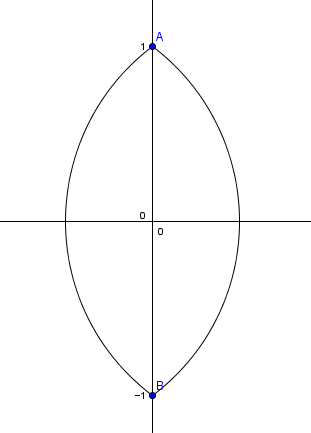
\includegraphics[scale=0.4]{1.png}
	\end{center}
\end{figure}

\longline

\subsection{using caption, label}
우선 문서의 앞부분에서 \textbackslash usepackage\{caption\}을 해준 다음,

다음과 같이 작성하면 그림 \verb+\+ref\{ding\_2\}과 같이 caption이 달린다.
\verb+\+begin\{figure\}

\verb+\+begin\{center\}

\verb+\+includegraphics[scale=0.4]\{2.png\}

\verb+\+captionsetup\{width=0.6\verb+\+textwidth\}

\verb+\+caption\{\verb+\+ding\}

\verb+\+label\{ding\_2\}

\verb+\+end\{center\}

\verb+\+end\{figure\}

다음과 같이 작성하면 Figure \ref{ding_2}과 같이 caption이 달린다.
\begin{figure}
	\begin{center}
		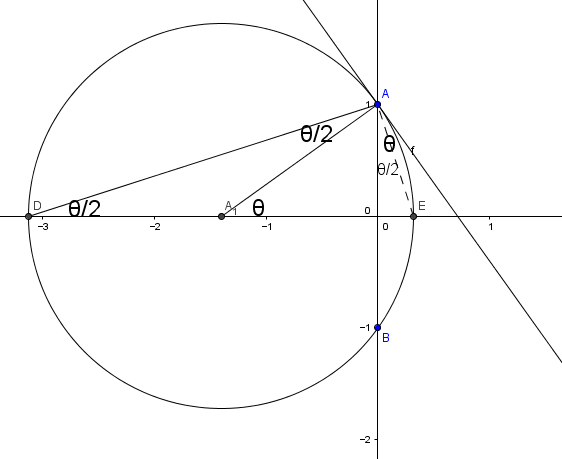
\includegraphics[scale=0.4]{2.png}
		\captionsetup{width=0.6\textwidth}
		\caption{\ding}
		\label{ding_2}
	\end{center}
\end{figure}

\begin{praise}
	참고로 TeXstudio에서는 \textbackslash includegraphics에서 그림 파일명에 마우스를 갖다대면 그림 미리보기가 나온다.
\end{praise}
\longline

\section{Other math functions}
\subsection{Matrix}

\$A = \verb+\+left[ \verb+\+begin\{array\}\{ccc\}

1 \& 2 \& 3\verb+\+\verb+\+

4 \& 5 \& 6\verb+\+\verb+\+

7 \& 8 \& 9\verb+\+\verb+\+

10 \& 11 \& 12

\verb+\+end\{array\}

\verb+\+right]\$

$A = \left[ \begin{array}{ccc}
1 & 2 & 3\\
4 & 5 & 6\\
7 & 8 & 9\\
10 & 11 & 12
\end{array}
\right]$

\longline
\subsection{Pile}
\$\$

f(x) = \verb+\+left\verb+\+\{

\verb+\+begin\{array\}\{ll\}

1,\&x=3\verb+\+\verb+\+

2,\&x\verb+\+ne3

\verb+\+end\{array\}

\verb+\+right.

\$\$

$$
f(x) = \left\{
\begin{array}{ll}
1,&x=3\\
2,&x\ne3
\end{array}
\right.
$$

\longline
\section{Troubleshooter}
\subsection{Compile Error}
tex 문서가 컴파일되지 않는 경우에는 다음이 가능하다.
\subsubsection{Grammar error}
grammar error를 고쳐준다.
특히, 수학 전용 수식 명령어가 포함되어 있는데 수식 시작부분과 끝부분에 \$를 넣지 않았다면 넣어주도록 한다. 
\subsubsection{Can't write on file}
Windows의 경우 OS 특성상 파일이 한 곳에서 이미 열려있을 경우 다른 곳에서 수정이 불가능하다.
pdf파일을 닫고 다시 컴파일을 시도하도록 한다.


\subsection{Broken text}
\subsubsection{Ref[?]}
reference 기능을 사용할 때 컴파일 후 pdf 파일을 확인하면 대괄호 안에 ?가 되어있을수 있다. 이는 수정된 문서를 최초로 컴파일했을때의 문제로, 컴파일을 한번 더 해주면 해결된다.
\subsubsection{글자가 없는 경우}
$\sim$ 와 같은 문자는 아무 생각 없이 그대로 넣어버리곤 한다. 그러면 글자가 나오지 않는다. 
\$\verb+\+sim\$ 와 같이 넣어주도록 하자.


\subsection{Label}
\verb+\+begin\{figure\}[h]

\verb+\+begin\{center\}

\verb+\+includegraphics[scale=0.5]\{Taxicab Hyperbola.png\} 

\verb+\+caption\{2차원 택시 쌍곡선\}\verb+\+label\{fig2\}

\verb+\+end\{center\}

\verb+\+end\{figure\}

와 같이 사진 이름에 공백이 있으면 사진 이름이 같이 나오는 버그 발생.

\section{Other useful tips}
\subsection{Using \textbackslash newcommand}
지난 2014 기초 R\&E논문작성 때 Taxicab Hyperbolloid를 여러번 쓰느라고 고생했었다.
하지만 \textbackslash ding 을 써주기만 하면 다음과 같이 나온다. 
문서의 앞부분에 \verb+\+newcommand\{\verb+\+ding\}\{\verb+\+textit\{Taxicab Hyperboloid\}\} 와 같이 써주어야 한다. 
\ding

\subsection{TeXstudio - \textquoteleft Convert to LaTeX\textquoteright}
TeX에 \textgreater 와 같은 문자를 쓸 때 그냥 쓰면 깨지거나 에러가 난다. 따라서 일일이 \textbackslash textgreater와 같이 변환해 주어야 된다. (심지어 방금 본 \textbackslash 도 \textbackslash textbackslash 와 같이 써야 된다! 부들부들)

특히 정보 R\&E의 경우 코드를 논문에 넣어야 하는 경우가 많은데, 각종 특수문자들을 일일이 LaTeX의 양식에 맞게 고치는 것이 매우 귀찮다!

\begin{praise}
	Dev-C++에서는 'Export'-'to TeX' 기능이 있다. 기능을 실행하면 cpp파일과 동일한 폴더에 tex파일이 하나 생겨 있을 것이며, 그를 compile하면 Dev-C++ IDE에서 보았던 그대로 코드가 나온다.\label{Dev-C++}
\end{praise} 

하지만 찬양 \ref{Dev-C++}와 같은 방법을 추천하지는 않는다. 코드 중 한 줄이 길어지게 될 경우 논문에서 잘리며(...), 필요 없이 코드에 색다른 폰트와 색을 넣어 놓는다. (코드의 가독성을 위해 색이 있어야 하는 것 아니냐고 할 수도 있지만, 코드가 쉬워 보이게 된다는 단점이 있...다고 하는 분들도 계시다.ㅁㄴㅇㄹ) 그러기 위해 수없이 많은 package들을 include해야 되게 되므로 compile시간이 길어진다. 찬양 \ref{Dev-C++}와 같은 방법을 사용하게 될 경우 코드는 가장 마지막에 넣도록 하자.

koTeX의 경우 \textbackslash usepackage[hangul]\{kotex\}과 Dev-C++에서 자동변환할 때 사용하는 package중 하나인 \textbackslash usepackage[ansinew]\{inputenc\}와 상충한다. 이는 ansinew가 kotex과 충돌해서 그런데, 정확한 메커니즘은 모르겠으나 대충 유니코드 충돌 문제가 아닌가 추측된다. 해결 방법은 해당 package를 포함시키지 않거나 ansinew를 utf8로 바꾸면 정상적으로 컴파일된다. 다만 이에 대한 부작용은 아직 겪어보지 않아서 모른다. 유의하자.

또, 개인적인 의견이지만 TeXstudio에서 ttfamily(코드를 처리하는 float environment 부분)를 접어놓아도 그 앞에서 \$를 추가할 때 자꾸 ttfamily 안의 \$와 반응하여 접어놓은게 풀린다. 이걸 어떻게 직접적으로 막을 수 있는지는 모르겠지만 Windows 운영체제에서의 TeXstudio 기준으로 Ctrl+Shift+M은 \$ \$를 추가해주므로 해당 문제를 우회할 수 있다. 꼭 이쪽이 아니더라도 유용한 단축키이다.

\begin{praise}
	TeXstudio의 또하나 편한 기능이 일일이 textbackslash할필요 없이 Idefix-Convert to LaTeX 기능을 쓰면 이것처럼 바로 변환해줌.
\end{praise}
...더이상 말이 필요한가요. texWorksEditor 말고 TeXstudio를 사용합시다 여러분



%\subsection{pointer}

%\subsubsection{pointer}
%asdf(1)
%\subsubsection*{what is this?}
%asdf(2)
%\subsubsection{Without numbering...}
%asdf(3)
% 안타깝게도 TeX에서는 다른 언어와 같이 /* ... */를 통해 일괄적으로 주석처리 되는 기능이 없다.

\section{Appendix}
\subsection{Fonts}
\begin{table}[!ht]
	\begin{center}
		\begin{tabular}{cccc}
			\hline
			\textbackslash textrm\{...\}&textrm{roman}&\textbackslash textsf\{...\}&textsf{Sans serif}\\
			
			\textbackslash texttt\{...\}&texttt{typewriter}&&\\
			
			\textbackslash textmd\{...\}&textmd{medium}&\textbackslash textbd\{...\}&textbd{bold face}\\
			
			\textbackslash textup\{...\}&textup{upright}&\textbackslash textit\{...\}&textit{italic}\\
			
			\textbackslash textsl\{...\}&textsl{slanted}&\textbackslash textsc\{...\}&textsc{SMALL CAPS}\\
			
			\textbackslash emph\{...\}&emph{emphasized}&\textbackslash textnormal\{...\}&textnormal{document font}\\
			
			
			\hline
		\end{tabular}
		\label{Fonts}
	\end{center}
\end{table}

\subsection{Absolute Font Size in Standard Classes}
\begin{table}[!ht]
	\begin{center}
		\begin{tabular}{cccc}
			\hline
			size&10pt\{default\}&11pt option&12pt option\\
			\textbackslash tiny&5pt&6pt&6pt\\
			\textbackslash scriptsize&7pt&8pt&8pt\\
			\textbackslash footnotesize&8pt&9pt&10pt\\
			\textbackslash small&9pt&10pt&11pt\\
			\textbackslash normalsize&10pt&11pt&12pt\\
			\textbackslash large&12pt&12pt&14pt\\
			\textbackslash Large&14pt&14pt&17pt\\
			\textbackslash LARGE&17pt&17pt&20pt\\
			\textbackslash huge&20pt&20pt&25pt\\
			\textbackslash Huge&25pt&25pt&25pt\\
			\hline	
		\end{tabular}
		\label{Fonts and its Sizes}
	\end{center}
\end{table}
\end{document}
